\documentclass[12pt]{article}
   
   \usepackage[utf8]{inputenc}
   \usepackage{graphicx}
   \usepackage{float}
   \usepackage{subcaption}
   \usepackage{mathtools}
   \usepackage{amsmath}
   \usepackage{amsfonts}

   \addtolength{\hoffset}{-0.7in}
   \addtolength{\textheight}{1.5in}
   \addtolength{\textwidth}{1.5in}
   \addtolength{\voffset}{-1in}
 
\title{EE 234: Experiment - 2 \\
       Open Circuit (OC) and Short Circuit (SC) Tests\\ on Single
Phase Transformer}
       
\author{Group-8 \\Gardas Chaitanya, 180070021  \\
Karthik Gvb, 180070022 \\
Hitesh Kandala, 180070023}
\date{\today}
%________________________________________________________________________________________________
\begin{document}

  \maketitle
  
    \section{Overview of the Experiment}
        \subsection{Aim}
        \begin{itemize}
            \item To understand the basic working principle of a transformer.
            \item To obtain the equivalent circuit parameters from OC and SC tests, and to estimate efficiency & regulation at various loads.
        \end{itemize}
        \subsection{Theory}
        \subsubsection{Open Circuit(OC) Test}
            Open circuit test or no load test on a transformer is performed to determine 'no load loss (core loss)' and 'no load current $I_o$'. Usually high voltage (HV) winding is kept open and the low voltage (LV) winding is connected to its normal supply.
            \begin{figure}[H]
                \centering
                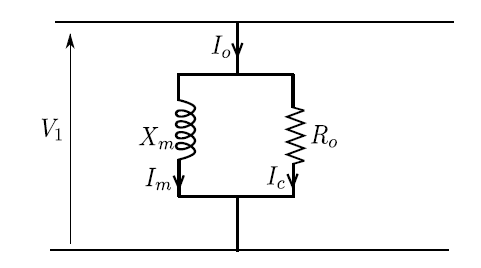
\includegraphics[width = 0.6\linewidth, height=2in]{LAB-2/OC_EQC.PNG}
                \caption{Equivalent circuit on OC test}
            \end{figure}
            
             $$cos\zeta=\dfrac{P_i}{V_1I_o}$$
             Hence, considering the circuit in Fig.1,$$I_c=I_ocos\zeta\\
             \Rightarrow R=\dfrac{V_1}{I_c}$$ $$I_m=I_osin\zeta\\
             \Rightarrow X_m=\dfrac{V_1}{I_m}$$
            \begin{figure}[H]
                \centering
                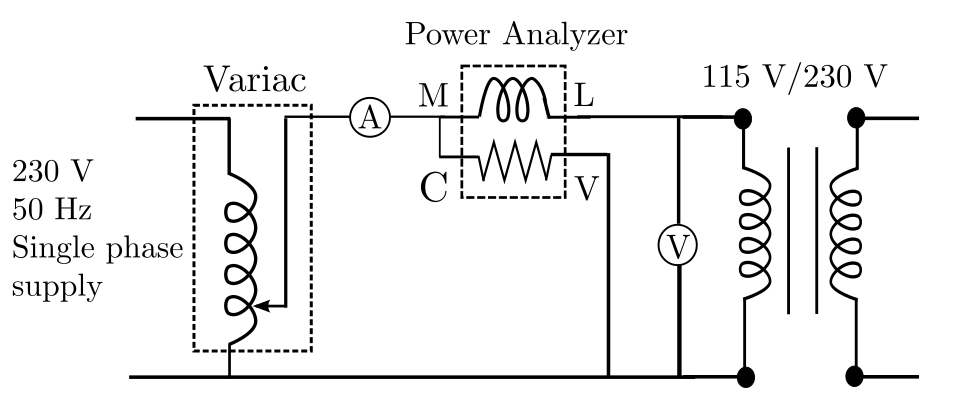
\includegraphics[width = 0.6\linewidth, height=2in]{LAB-2/oc.png}
                \caption{Connection diagram for OC test}
            \end{figure}
            
            % \begin{equation}
                
            % \end{equation}
            
        \subsubsection{Short Circuit(SC) Test}
            The test is conducted on the high-voltage (HV) side of the transformer where
            the low-voltage (LV) side or the secondary is short circuited. A wattmeter is
            connected to the primary. An ammeter is connected in series with the primary
            winding.
            \begin{figure}[H]
                \centering
                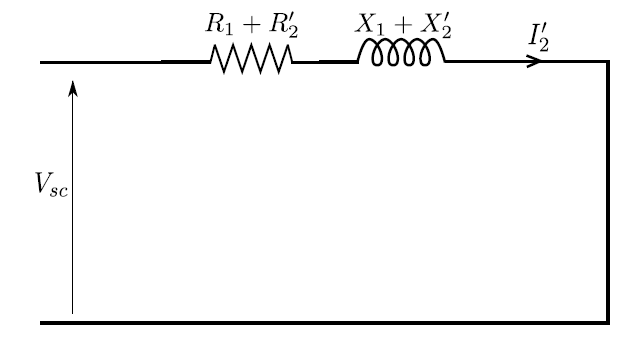
\includegraphics[width = 0.6\linewidth]{LAB-2/SC_EQC.PNG}
                \caption{Equivalent circuit on SC test}
            \end{figure}
            
            $$cos\theta=\dfrac{P_c}{V_{sc}I'_2}$$
            Hence, considering the circuit in Fig.2,$$Z_{sc}=\dfrac{V_{sc}}{I'_2}$$
            \begin{equation}
                 \Rightarrow(R_1+R_2')=Z_{sc}cos\theta
                    \quad\text{and}\quad 
                (X_1+X_2')=Z_{sc}sin\theta
            \end{equation}
            \begin{figure}[H]
                \centering
                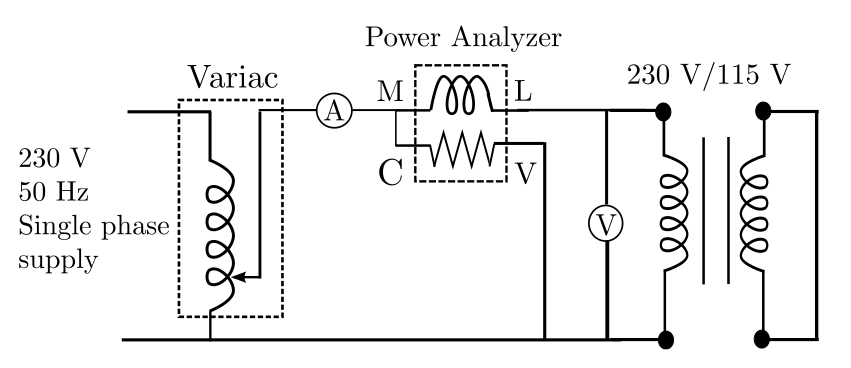
\includegraphics[width = 0.6\linewidth]{LAB-2/sc.png}
                \caption{Connection diagram for SC test}
            \end{figure}
            
        \subsubsection{Voltage Regulation}
            The voltage regulation of the transformer is the percent changein the output voltage from no-load to full-load. Voltage regulation is also influenced by power factor since it is the determining factor in the  secondary voltage.
            \begin{equation}
                 \% \text{regulation} = \frac{I'_2.R_{eq}.cos\phi \pm I'_2.X_{eq}.sin\phi}{V'_2}
            \end{equation}
            where, $I'_2 = $ load current,  $R_{eq} = R_1 + R'_2$,  $X_{eq} = X_1 + X'_2$,\\ \hspace{1cm} '+' sign for lagging pf \& '-' sign for leading pf
        \subsubsection{Efficiency}
            The efficiency of a transformer depends on its design and is equal to the power output divided by the power input. It is necessary to use higher efficiency at the higher power levels because the amount of energy wasted is significant.
            \begin{equation}
                 \eta = \frac{\text{output power}}{\text{input power}} = \frac{\text{output power}}{\text{output power + iron losses + copper losses}}
            \end{equation}
            \begin{equation}
                \eta = \frac{x.S.cos\phi}{x.S.cos\phi+P_i+P_c.x^2}
            \end{equation}
            where, S = rated VA of the transformer, x = fraction of full load, $\phi$ = load power factor angle
        
  \newpage
    \section{Observations}
        
        \subsection{OC test}
            
            \begin{table}[H]
                \centering
                \begin{tabular}{|c|c|}
                    \hline
                    Parameter & Value\\
                    \hline
                    Current($I_o$) & 295.6mA \\
                    Voltage($V_1$) & 114.5V \\
                    Power($P_i$) & 13.45W\\
                    \hline
                \end{tabular}
                \caption{OC test results}
                \label{tab:my_label}
            \end{table}
            
            \begin{figure}[H]
                \centering
                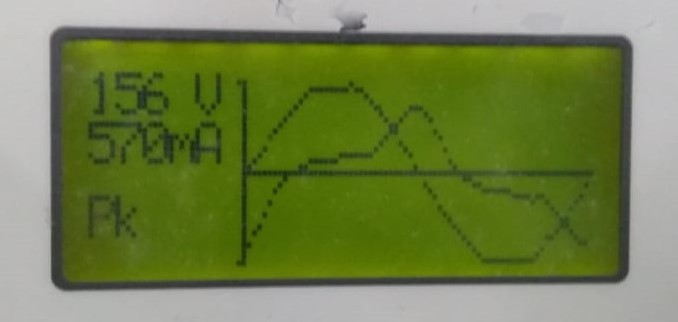
\includegraphics[width = 0.6\linewidth]{LAB-2/OC_test_waveforms1.jpeg}
                \caption{Current and Voltage waveforms across the supply side in OC test}
            \end{figure}
            
            \subsubsection{Core Parameters}
      
                $$cos\zeta=\dfrac{P_i}{V_1I_o}=\dfrac{13.45}{33.8462}=0.397$$
                Hence, considering the circuit in Fig.1,$$I_c=I_ocos\zeta\\
                \Rightarrow R=\dfrac{V_1}{I_c}=\dfrac{114.5}{0.117}=974.74\Omega$$ $$I_m=I_osin\zeta\\
                \Rightarrow X_m=\dfrac{V_1}{I_m}=\dfrac{114.5}{0.271}=422.11\Omega$$
            
        \subsection{SC test}
        
            \begin{table}[H]
                \centering
                \begin{tabular}{|c|c|}
                    \hline
                    Parameter & Value\\
                    \hline
                    Current($I'_2$) & 8.47A \\
                    Voltage($V_{sc}$) & 11.435V \\
                    Power($P_c$) & 89.47W\\
                    \hline
                \end{tabular}
                \caption{SC test results}
                \label{tab:my_label}
            \end{table}
            
            \subsubsection{Winding Parameters}
            From the experimental results,
            \vspace{-15pt}
            $$cos\theta=\dfrac{P_c}{V_{sc}I'_2}=\dfrac{89.47}{96.85}=0.924$$
            Hence, considering the circuit in Fig.2,$$Z_{sc}=\dfrac{V_{sc}}{I'_2}=\dfrac{11.435}{8.47}=1.35\Omega$$
            \begin{equation}
                 \Rightarrow(R_1+R_2')=Z_{sc}cos\theta=1.247\Omega
                    \quad\text{and}\quad 
                (X_1+X_2')=Z_{sc}sin\theta=0.517\Omega
\end{equation}
        \subsection{Regulation}
           
            \begin{table}[H]
                \centering
                \begin{tabular}{|c|c|c|c|}
                \hline 
                    Load(\%) & Pf = 0.6 lead & Pf = 0.6 lag & Pf = 1 \\\hline
                    25 & 0.316 & 1.098 & 1.179 \\\hline
                    50 & 0.632 & 2.196 & 2.357 \\\hline
                    75 & 0.949 & 3.294 & 3.536 \\\hline
                    100 & 1.265 & 4.392 & 4.714 \\\hline
                \end{tabular}
                \caption{Regulation values for different loads and power factors}
            \end{table}  
            
            \begin{figure}[H]
                \centering
                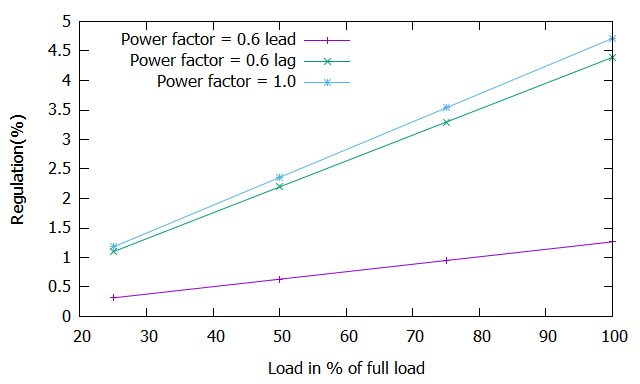
\includegraphics[width = \linewidth]{LAB-2/Regu_vs_load.png}
                \caption{Regulation vs Load for different power factors}
            \end{figure}
                
        \subsection{Efficiency}
        
              \begin{table}[H]
                \centering
                \begin{tabular}{|c|c|c|c|}
                \hline
                    Load(\%) & Pf = 0.6 lead & Pf = 0.8 lag & Pf = 1 \\\hline
                    25 & 93.943 & 95.387 & 96.275 \\\hline 
                    50 & 94.19 & 95.577 & 96.4298 \\\hline
                    75 & 93.12 & 94.75 & 95.755 \\\hline
                    100 & 91.76 & 93.69 & 94.888 \\\hline
                \end{tabular}
                \caption{Efficiency values for different loads and power factors}
            \end{table}  
            
            \begin{figure}[H]
                \centering
                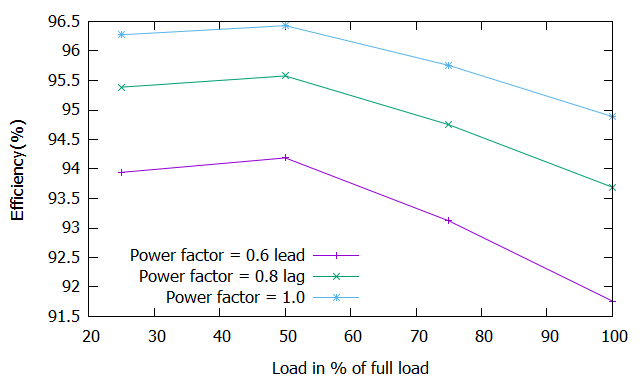
\includegraphics[width = \linewidth]{LAB-2/Eff_vs_LoVA.png}9+
                \caption{Efficiency vs Load for different power factors}
            \end{figure}
    
   % \section{Conclusion}
        
    %    The significant things that we have learned through this experiment were the way the 
  \newpage
  
  \section{Post-lab Questions}
  
    
    1. Which winding ( LV or HV) should be kept open while conducting OC test? Justify your answer.
    \vspace{0.1cm} \\
    \textbf{Ans} The HV winding should be kept open while conducting OC test.\\
    In case if we connect the supply to the HV side and open the LV side there could be two problems:
    \begin{itemize}
        \item In OC test, rated voltage has to be applied to whichever side the supply is connected and on HV side as the name suggests a \textbf{high voltage} is needed to operate it at it's rating point which may not be available at the instant.
        \item Also the current which is needed to be measured on the supply side(HV side) would be very small, small enough for the usual watt meters unable to detect. Hence we would be recquiring a watt meter which measures very high voltages and also \textbf{very small currents} which are hard to be available.    
    \end{itemize}
    2. Assume that the given transformer has the following name plate ratings:
    40 kVA, 440 V/11 kV, 50 Hz. What do these numbers imply?
    \vspace{0.1cm} \\
    \textbf{Ans} 40 kVA denotes the rated apparent power of the transformer. It resembles the size and capacity of transformer.\\
    440V/11kV denotes that primary side is rated 440V and secondary is rated 11kV.\\
    50Hz denotes the rated frequency of the transformer. Operating the transformer at a lower frequency will increase the coreflux leading to magnetic saturation and overheating due to eddy currents and hysterisis loss.\vspace{0.2cm} \\
    3. Comment on the nature of the current waveform drawn from the source during OC test for (i)
    50\%, (ii) 100\% and (iii) 110\% of the rated voltage.
    \vspace{0.1cm} \\
    \textbf{Ans} The current depends on the flux in the coil. This flux developed due to the
applied voltage. At the 50percent rated voltage, the sinusoidal input produces
sinusoidal current waveform. But at higher voltages, such as at 100percent,
110percent, we observe a distortion. This is because, the relation between the
current and flux is non linear for higher values. \vspace{0.2cm}\\
    4. Can the regulation be negative? What does it signify?
    \vspace{0.1cm} \\
    \textbf{Ans} Regulation can be negative, 
    \begin{equation}
        Voltage \ regulation \ \% = \frac{V_{NL} - V_{FL}}{V_{FL}}\times 100
    \end{equation}
    $V_{NL}$ and $V_{FL}$ are secondary terminal no load and full load voltages at same primary voltage
    negative regulation implies that there is voltage rise instead of voltage drop as approaching secondary terminals from primary terminals at full load, this is possible for certain \textbf{capacitive loads}. Hence negative regulation implies that the load has leading power factor \vspace{0.2cm} \\
     5. Assume that you have been given a transformer manufactured in the US ( The supply voltage
    and frequency are 110 V and 60 Hz respectively). What voltage will you apply if this transformer
    is to be used in this country? Justify your answer.
    \vspace{0.1cm} \\
    \textbf{Ans} The rated voltages are determined such that the core operates at its saturation point, i.e at the core's saturation flux density. If this is increased by some means,\textbf{ over fluxing} of the core occurs and the extra flux leaks out into air or lamination parts heating them up which results in the damage of the transformer.\\
    Flux is directly proportional to the voltage applied and \textbf{inversely proportional to the frequency}. So applying the same voltage at lower frequency might damage the transformer, hence voltage $\leq 84V$ is feasible to apply. \vspace{0.2cm}\\
   % 6. What is the reason for high no load current at lower-than-rated voltage for the no load test on
   % high frequency transformer which was demonstrated to you by the Ta's ?
    %\vspace{0.1cm} \\
    %\textbf{Ans} \vspace{0.2cm}\\
    6. Assume that you have been given two transformers of identical VA, and voltage ratings. But one
    of them is a 10 kHz transformer and another is a 100 Hz transformer. Just by inspection, how
    would you identify which one is the high frequency transformer? Justify your answer.
    \vspace{0.1cm} \\
    \textbf{Ans} The saturation operating points would be same assuming similar core is used in both the transformers, also flux is directly proportional to the voltage applied and inversely proportional to the frequency and number of turns. So for the same voltage ratings the one with high frequency has \textbf{lesser number of turns} on both sides.\vspace{0.2cm}\\
    7. What is an `impedance matching' transformer? Name one instrument of everyday use, in which
    this transformer being used.
    \vspace{0.1cm} \\
    \textbf{Ans} In power optimization problems one might come across the requirement of equalising input impedance and load impedance which may not be possible by adding an impedance in series or in parallel. In such cases one can use a typical transformer with adjusted turns ratio such that the impedances are matched. \\
    \textbf{Audio amplifiers} use impedance matching transformers to match speaker impedance and to the input impedance.
\end{document}